% 符号终态核对小样（对照④）：我方数学栈（amsmath＋unicode-math＋TeX Gyre Termes Math）
% 逐符号渲染，与教材同符号真迹并排（教材侧裁片由 _sym_board.py 注入）
% ⌒：教材 190 页无 U+2312 字符实例（只列不改，看 Termes Math 侧兜底形态）
\documentclass[fontset=none]{ctexart}
\setmainfont{Times New Roman}
\setCJKmainfont[Path=C:/Users/28120/AppData/Local/Microsoft/Windows/Fonts/,BoldFont=FZHei-B01S.ttf]{FZShuSong-Z01S.ttf}
\usepackage{amsmath}
\usepackage{unicode-math}
\setmathfont{texgyretermes-math.otf}
\usepackage{tikz}
% E 版 \parallel（与 qp-fonts.tex \AtBeginDocument 同一落法定义，保真起见在此直接内联）
\newcommand{\qppar}{\mathrel{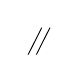
\begin{tikzpicture}[x=1em,y=1em,baseline={(0,0)}]
  \fill (-0.412,-0.016) -- (-0.375,-0.016) -- (0.114,0.956) -- (0.077,0.956) -- cycle;
  \fill (-0.115,-0.016) -- (-0.078,-0.016) -- (0.411,0.956) -- (0.374,0.956) -- cycle;
\end{tikzpicture}}}
\renewcommand{\parallel}{\qppar}
\begin{document}\fontsize{10.09pt}{18.25pt}\selectfont
\begin{enumerate}
\item 夹角：\(\angle AOB\)，记作\(\langle\overrightarrow{a},\overrightarrow{b}\rangle\)
\item 垂直：\(\overrightarrow{a}\perp\overrightarrow{b}\)，\(\overrightarrow{OA}\perp\overrightarrow{OB}\)
\item 平行：\(\overrightarrow{a}\parallel\overrightarrow{b}\)（E 版 TikZ 复刻平行号）
\item 箭头：\(\overrightarrow{a}\)，\(\overrightarrow{AB}\)，\(\overset{\scriptscriptstyle\rightharpoonup}{a}\)（备看），字面\(\mathord{→}\)
\item 弧：\(\overparen{AB}\)（U+23DC 途径），字面⌒（U+2312 直排兜底形态）
\end{enumerate}
\end{document}
